\documentclass[../../Cours_M1.tex]{subfiles}
\newcommand{\nomTD}{TP2 : Asservissement échantillonné, méthode de ZDAN}
\renewcommand{\nomentete}{UE421-\nomTD}
\renewcommand{\auteur}{Aymeric Arnould, Tom Colinot}
\newcommand{\z}{z^{-1}}

\begin{document}
\section*{\nomTD}

\subsection*{I/ Introduction et Préparation}

On souhaite corriger par la méthode de ZDAN le processus de fonction de transfert \[G(p) = \frac{K}{1+\tau p}\]

\begin{figure}[h!]
\centering
\begin{tikzpicture}
\sbEntree{E}
\sbComp{comp}{E}                
\sbRelier[$E(z)$]{E}{comp}
\sbBloc{reg}{$D(z)$}{comp}  
\sbRelier[$\epsilon$]{comp}{reg}
\sbBloc{boz}{Bloqueur $B_0(p)$}{reg}      
\sbRelier{reg}{boz}
\sbBloc{sys}{$G(p)$}{boz}
\sbRelier{boz}{sys}
\sbSortie{S}{sys}                
\sbRelier[$S(p)$]{sys}{S}
\sbDecaleNoeudy[4]{S}{R}
\sbBlocr[7]{can}{Échantillonneur}{R}
\sbRelieryx{sys-S}{can}
\sbRelierxy{can}{comp}
\end{tikzpicture}
\caption{Asservissement considéré}
\end{figure}

\subsubsection*{Préparation 1}

On cherche à expliciter la fonction de transfert en $z$ du processus \[G(p) = \frac{K}{1+\tau p}\]

Ce processus est associé au bloqueur d'ordre 0 modélisé par \[B_0(p) = \frac{1-e^{-T_ep}}{p}\]

\begin{align*}
H(z) & = Z\{B_0(p)G(p)\} = (1-\z)Z\{^*L^{-1}\{\frac{G(p)}{p}\}\} \\
& = (1-\z)Z\{^*L^{-1}\{ \frac{K}{p(1+\tau p)} \} \\
& = K (1-\z)Z\{^*L^{-1}\{ \frac{1}{p} - \frac{\tau}{1+\tau p} \} \\
& = K (1-\z)Z\{1-e^{-\frac{nT_e}{\tau}}\} \\
& = K (1-\z)(\frac{z}{z-1}-\frac{z}{z-D}) \text{ où } D = e^{-T_e/\tau} \\
& = K(1-\frac{z-1}{z-D}) \\
H(z) & = K(1-D)\frac{\z}{1-D\z}
\end{align*}
\[ \boxed{H(z) = k_1\frac{\z}{1-a\z} \avec k_1 = K(1-e^{-\frac{T_e}{\tau}}) \et a = e^{-\frac{T_e}{\tau}}} \]

\subsubsection*{Préparation 2}

On utilise un correcteur de la forme :
\[ D(z) = K_d\frac{1-a\z}{(1-\z)(1+b\z)} \]

\begin{itemize} \setlength{\itemsep}{10mm}
\item \textbf{Calcul de la fonction de transfert en boucle fermée }

En boucle ouverte,
\[ T_{BO}(z) = D(z)H(z) = k_1K_d \frac{\z}{(1-\z)(1+b\z)} \]

On a donc en boucle fermée :
\begin{align*}
F(z) & = \frac{T_{BO}(z)}{1+T_{B0}(z)} \\
& = \frac{k_1K_d\z}{(1-\z)(1+b\z) +k_1K_d\z} \\
& = \frac{k_1K_d\z}{1+\z(k_1K_d+b-1)-bz^{-2}}
\end{align*}

\item \textbf{Erreur statique de position}

En utilisant le théorème de la valeur finale, avec une entrée échelon $E(z) = E_0 \frac{z}{z-1}$,

\begin{align*}
\lim_{t\rightarrow +\infty}s(t) & = \lim_{z\rightarrow 1} \frac{z-1}{z} F(z) \frac{z}{z-1}E_0 \\
& = \lim_{z\rightarrow 1} \frac{k_1K_d\z}{1+\z(k_1K_d+b-1)-bz^{-2}} E_0 \\
& = \frac{k_1K_d}{1+(k_1K_d-1+b)-b}E_0 \\
& = E_0
\end{align*}

On a donc bien une erreur statique de position nulle.

\item On écrit la fonction de transfert en boucle fermée sous la forme suivante :
\[ \boxed{ F(z) = \frac{A\z}{1+B\z+Cz^{-2}} \avec A = k_1K_d, \quad B=k_1K_d + b -1, \quad C = -b }\]
\end{itemize}

\subsubsection*{Préparation 3}
\begin{itemize}\setlength{\itemsep}{10mm}

\item On veut la fonction de transfert du second ordre :
\[ M(p) = \frac{F_0}{1+\frac{2m}{\Omega}p+\frac{p^2}{\Omega^2}} = \frac{\omega_0}{(p+x)^2 + \omega_0^2} = \frac{\frac{\omega_0}{\omega_0^2+x^2}}{\frac{p^2}{\omega_0^2+x^2}+\frac{2x}{\omega_0^2 + x^2}p +1}\]

On en déduit donc : \[ \boxed{ F_0 = \frac{\omega_0}{\omega_0^2 + x^2}, \quad \Omega = \sqrt{\omega_0^2 + x^2} \quad \et \quad m=\frac{x}{\Omega}} \]

\item \[ \boxed{x = m\Omega, \quad \omega_0=\Omega\sqrt{1-m^2} \text{ pour } m< 1 } \]

\item La transformée en $z$ de la fonction de transfert $M(p)$ est 
\[ M(z) = \frac{ze^{-xT_e}\sin(\omega_0T_e)}{z^2 - 2ze^{-xT_e}\cos(\omega_0T_e)+e^{-2xT_e}} \]

Le dénominateur a pour déterminant $\Delta = 4e^{-2xT_e}(\cos^2(\omega_0T_e)-1) \leq 0$.

Les pôles sont donc \[z_{1,2} = e^{-xT_e}(\cos(\omega_0T_e) \pm j \sqrt{1-\cos^2(\omega_0T_e)}) = e^{-xT_e\pm j\omega_0T_e}\]

\item On veut que $M(z)$ et $F(z)$ aient les mêmes pôles :
\[ \frac{A\z}{1+B\z+Cz^{-2}} = \frac{ze^{-xT_e}\sin(\omega_0T_e)}{z^2 - 2ze^{-xT_e}\cos(\omega_0T_e)+e^{-2xT_e}} = \frac{\z e^{-xT_e}\sin(\omega_0T_e)}{1 - 2\z e^{-xT_e}\cos(\omega_0T_e)+z^{-2}e^{-2xT_e}} \]

Donc en identifiant :
\[ \boxed{ A = e^{-xT_e}\sin(\omega_0T_e), \quad B = -2 e^{-xT_e}\cos(\omega_0T_e), \quad C = e^{-2xT_e}} \]

\item On a immédiatement
\[ \boxed{ b = -e^{-2xT_e}} \]

De plus, $B = k_1K_d + b -1 = -2 e^{-xT_e}\cos(\omega_0T_e)$ donc 
\[ \boxed{ K_d = \frac{1-2 e^{-xT_e}\cos(\omega_0T_e)+e^{-2xT_e}}{k_1} }\]
\end{itemize}

\subsubsection*{Préparation 4}

\begin{itemize}\setlength{\itemsep}{10mm}
\item On a le correcteur 
\[ D(z) = \frac{K_d-K_da\z}{1+(b-1)\z -bz^{-2}} = \frac{Y(z)}{X(z)} \]
On transforme cette expression en équation de récurrence :
\[Y(z)(1+(b-1)\z -bz^{-2}) = X(z)(K_d-K_da\z) \]
\[ \boxed{y[n] = K_dx[n] - K_d a x[n-1] + (1-b)y[n-1] + by[n-2]}\]

\item On en déduit donc : 
\[ \boxed{ A_1 = K_d, A_2 = -aK_d, B_1 = 1-b, B_2 = b } \]

\item Applications numériques :
\[ T_e = 50 \mu s, m = 0,5, \Omega = 5000 rad/s, \tau = 1ms, K=2 \]
\begin{multicols}{3}
$a = 0.9512$\\
$k_1 = 0.09754$\\
$x = 2500 $ rad/s\\
$\omega_0 = 4330 $rad/s\\

$A = 0.18957$\\
$B = -1.72379$\\
$C = 0.7788$\\
$b = -0.7788$\\
$K_d = 0.56397$\\
$A_1 = 0.56397$\\
$A_2 = -0.53645$\\
$B_1 = 1.7788$\\
$B_2 = -0.7788$
\end{multicols}

\item Avec un coefficient d'amortissement $m=0.5$, on détermine $t_r\Omega = 5.3$ donc $t_r = 1,26$ ms. Le premier dépassement est de $D_1 = 25 \%$.
\end{itemize}

\subsection*{II/ Manipulation}

\subsubsection*{Manipulation 1}

\textit{Simulation du système analogique} \\

Avec les valeurs calculées ci-dessus, en utilisant un pas d'intégration de $10^{-5}$s et un schéma d'Euler d'ordre 1, on obtient la réponse indicielle suivante :

\begin{figure}[h!]
\centering
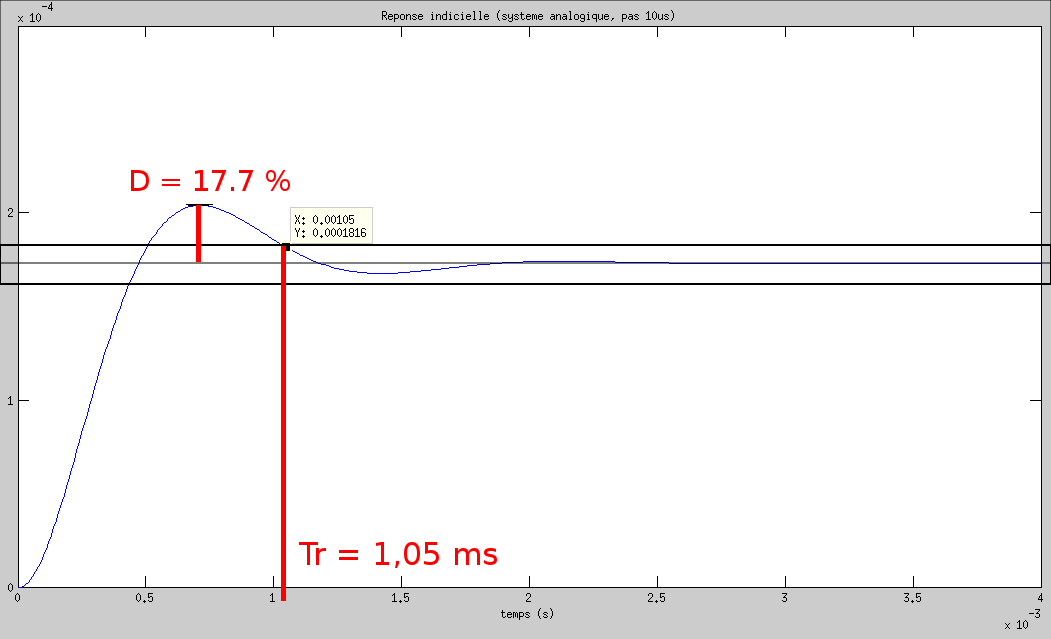
\includegraphics[scale=0.4]{analtr5.png}
\caption{Réponse indicielle du système analogique simulé}
\end{figure}

Si on diminue le pas d'intégration, alors la réponse calculée peut être très différente. Par exemple, avec un temps de $10^{-4}$ s, on a la réponse :

\begin{figure}[h!]
\centering
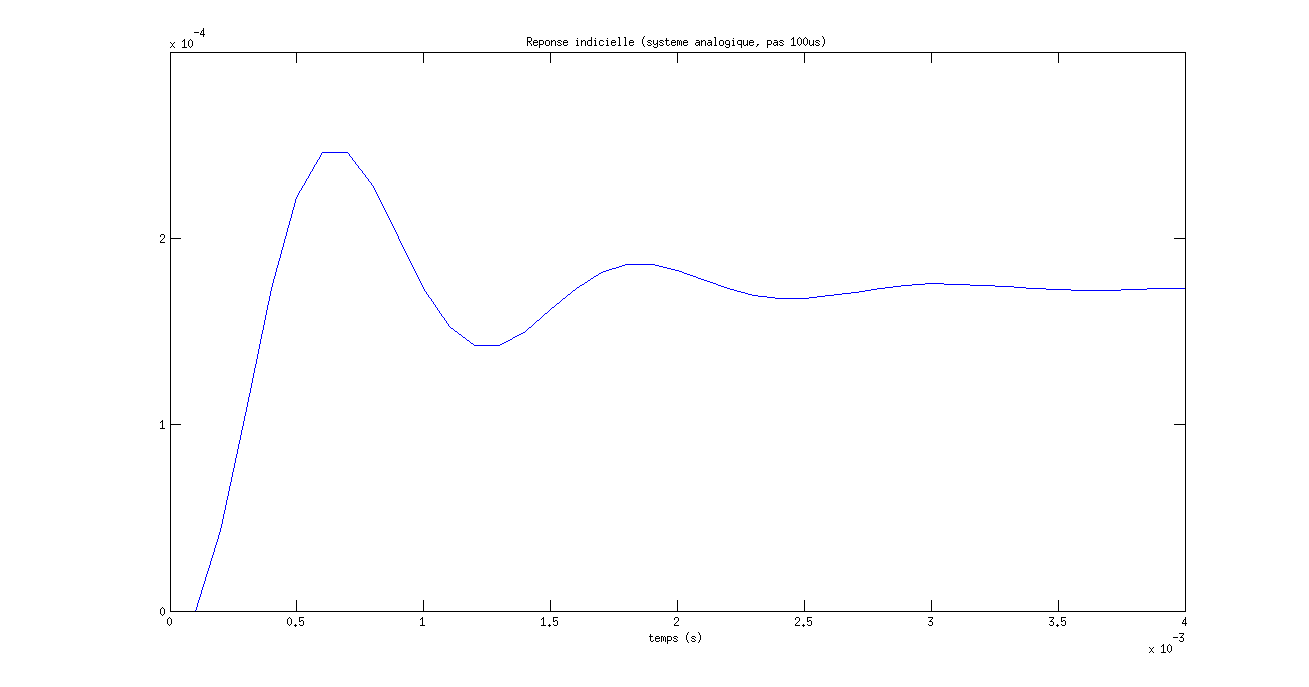
\includegraphics[scale=0.4]{analbullshit.png}
\end{figure}

Si on prend un schéma d'intégration plus précis, sans changer le pas d'intégration, on peut obtenir une réponse satisfaisante. Par exemple, en prenant un schéma de Dormand-Price d'ordre 8, on obtient la réponse suivante, qui est similaire à celle obtenue précédemment.

\begin{figure}[h!]
\centering
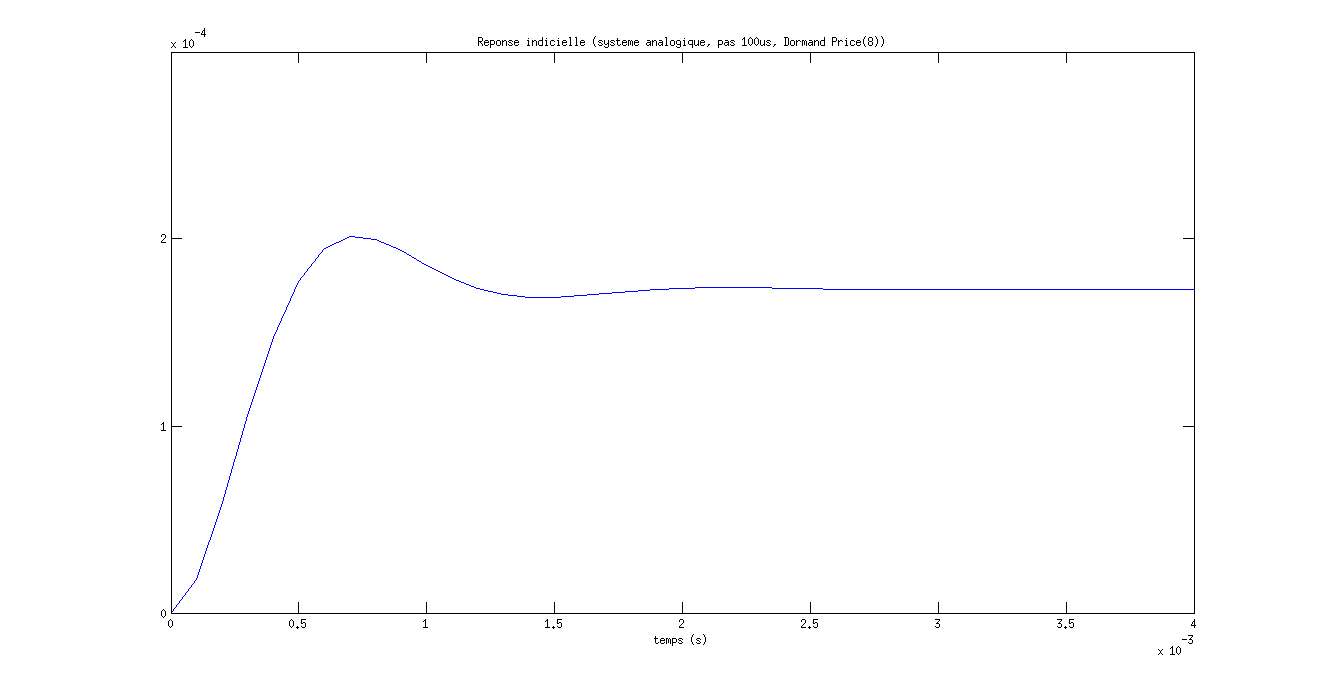
\includegraphics[scale=0.4]{anal_DP8.png}
\end{figure}

\textit{Simulation de l'asservissement avec un correcteur numérique}\\

On réalise l'asservissement avec le correcteur numérique. Les réponses du second ordre analogique et du second ordre numérique diffèrent d'un gain induit par l'échantillonnage. Pour les comparer, on peut donc les normaliser par leur gain statique.

\begin{figure}[h!]
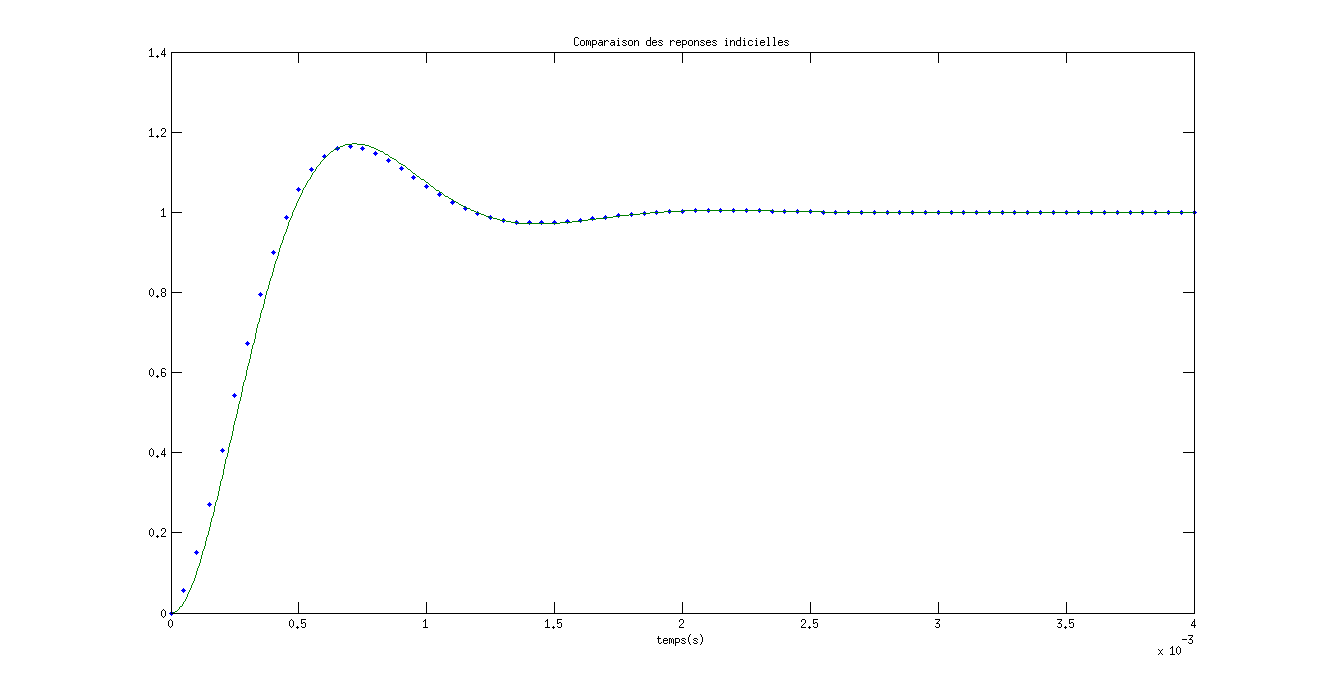
\includegraphics[scale=0.40]{anal_num.png}
\end{figure}

La réponse du système numérique est très proche de celle du système analogique, mais les courbes ne se superposent pas tout à fait.
\newpage

On réalise la simulation pour des valeurs différentes de $T_e$ :

\begin{figure}[h!]
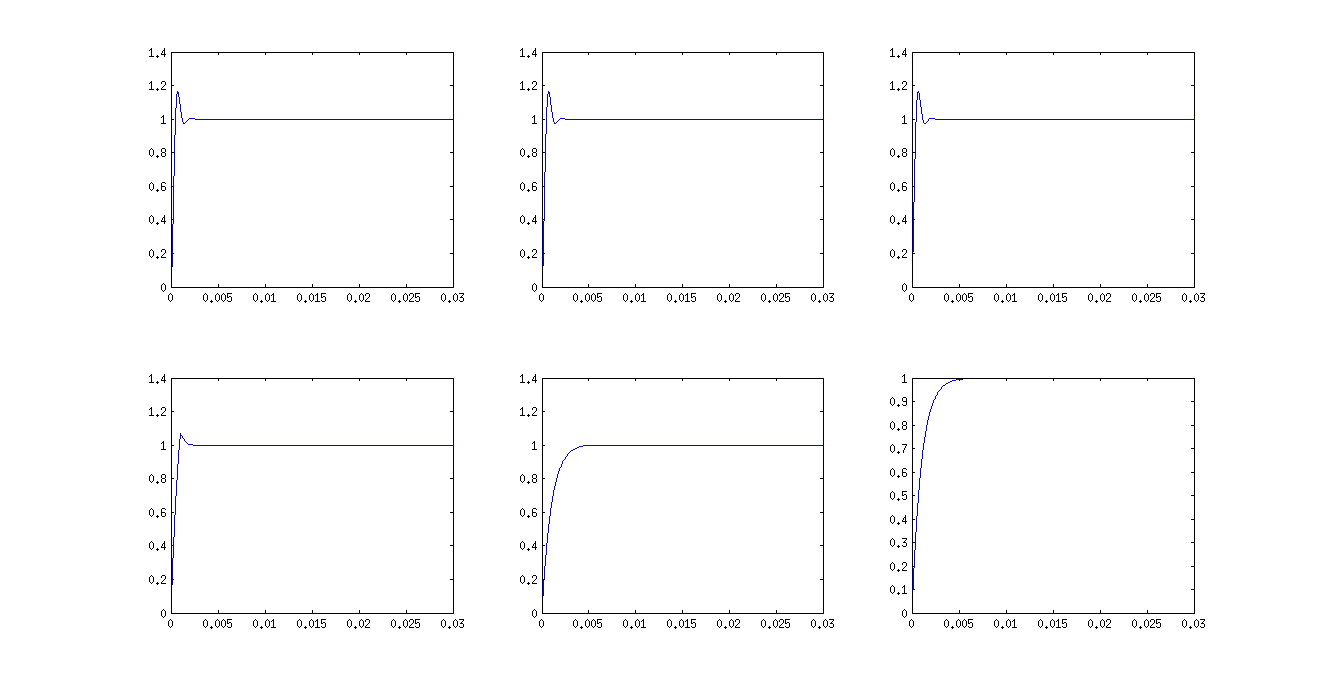
\includegraphics[scale=0.40]{num_Te.png}
\caption{Réponse de l'asservissement pour $T_e$ = 1$\mu$s,10$\mu$s,100$\mu$s,1ms,5ms,10ms}
\end{figure}

La variation de la période d'échantillonnage fait varier la valeur du premier dépassement. Lorsque $T_e$ augmente et se rapproche de la période de Shannon $\frac{\pi}{\Omega}$, le dépassement  diminue. \\

On avait remarqué que les réponses simulées avec $M(p)$ et $M(z)$ étaient légèrement différentes. Pour retrouver une réponse proche de celle de la boucle avec le correcteur numérique, en utilisant un modèle analogique, on approxime le bloqueur d'ordre zéro par un retard pur de $T_e/2$ et on utilise l'approximation de Tustin pour remplacer la fonction de transfert en $z$ par une fonction de transfert en $p$.

\noindent Remarque : on utilise les fonctions de Matlab pour faire l'approximation de Tustin.\\

\begin{figure}[h!]
\centering
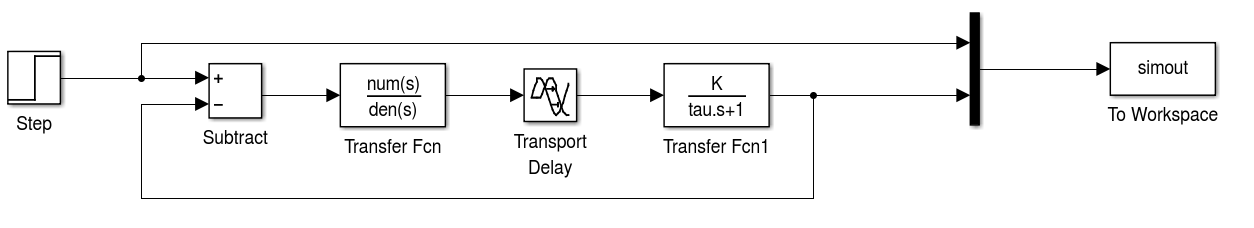
\includegraphics[scale=0.4]{tustin.png}
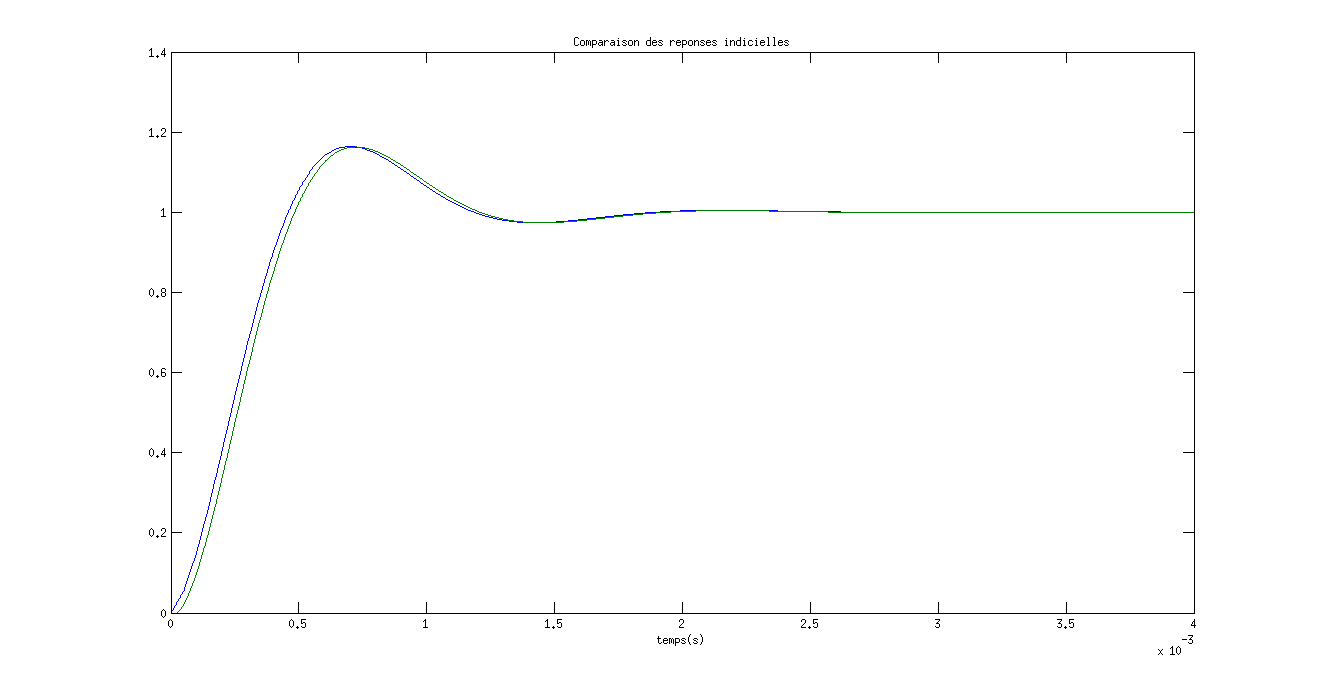
\includegraphics[scale=0.4]{simtustin.png}
\end{figure}

Les deux courbes ne sont pas superposées. L'approximation a cependant permis d'améliorer le modèle analogique vu au début du TP.

\subsubsection*{Manipulation 2}

Grâce à la carte D-space on a pu remplacer la partie analogique simulée du système par une partie analogique réelle. 

On retrouve bien les performances du système modélisé : $D = 17.3 \%$ et $t_5\% = 1 ms$ (voir figures en annexe).


\end{document}